
\documentclass{statsoc}

%\usepackage{hyperref}

\usepackage[a4paper]{geometry}
\usepackage{graphicx}
\usepackage[textwidth=8em,textsize=small]{todonotes}
\usepackage{amsmath}
\usepackage{bm}

%\usepackage[authoryear]{natbib}

\usepackage[hidelinks]{hyperref}

\usepackage{lineno}
\linenumbers	

\title[Mapping malaria by sharing spatial information]{Mapping malaria by sharing spatial information between incidence and prevalence datasets}
\author[Tim C.D. Lucas {\it et al.}]{Tim C.D. Lucas}
\address{Big Data Institute,
University of Oxford,
Oxford,
UK.}
\email{timcdlucas@gmail.com}
\author{Anita K. Nandi\textsuperscript{1}}
\author{Elisabeth G. Chestnutt\textsuperscript{1}}
\author{Katherine A. Twohig\textsuperscript{1}}
\author{Suzanne H. Keddie\textsuperscript{1}}
\author{Emma L. Collins\textsuperscript{1}}
\author{Rosalind E. Howes\textsuperscript{1}}
\author{Michele Nguyen\textsuperscript{1}}
\author{Susan F. Rumisha\textsuperscript{1}}
\author{Andre Python\textsuperscript{1}}
\author{Rohan Arambepola\textsuperscript{1}}
\author{Amelia Bertozzi-Villa\textsuperscript{1,2}}
\author{Penelope Hancock\textsuperscript{1}}
\author{Punam Amratia\textsuperscript{1}}
\author{Katherine E. Battle\textsuperscript{1}}
\author{Ewan Cameron\textsuperscript{1}}
\author{Peter W. Gething\textsuperscript{1, 3, 4}}
\author{Daniel J. Weiss\textsuperscript{1}}
\address{1. Big Data Institute,
University of Oxford,
Oxford,
UK.}
\address{2. Institute for Disease Modeling, Bellevue, WA, USA}
\address{3. Telethon Kids Institute, Perth Children’s Hospital, Perth, Australia}
\address{4. Curtin University, Perth, Australia}

% Title must be 250 characters or less.

%*\textsuperscript{1}, Anita Nandi\textsuperscript{1}, Michele Nguyen\textsuperscript{1}, Susan Rumisha\textsuperscript{1}, Rosalind Howes\textsuperscript{1}, Katherine E. Battle\textsuperscript{1}, Penelope Hancock\textsuperscript{1}, Andre Python\textsuperscript{1}, Ewan Cameron\textsuperscript{1}, Pete Gething\textsuperscript{1} and Daniel J. Weiss\textsuperscript{1}





\begin{document}


% Please keep the abstract below 300 words
\begin{abstract}
As malaria incidence decreases and more countries move towards elimination, maps of malaria risk in low prevalence areas are increasingly needed.
For low burden areas, disaggregation regression models have been developed to estimate risk at high spatial resolution from routine surveillance reports aggregated by administrative unit polygons.
However, in areas with both routine surveillance data and prevalence surveys, models that make use of the spatial information from prevalence point-surveys might make more accurate predictions.
Using case studies in Indonesia, Senegal and Madagascar, we compare the out-of-sample mean absolute error for two methods for incorporating point-level, spatial information into disaggregation regression models.
The first simply fits a binomial-likelihood, logit-link, Gaussian random field to prevalence point-surveys to create a new covariate.
The second is a multi-likelihood model that is fitted jointly to prevalence point-surveys and polygon incidence data.
We find that in most cases there is no difference in mean absolute error between models.
In only one case did the new models performed the best.
More generally, our results demonstrate that combining these types of data has the potential to reduce absolute error in estimates of malaria incidence but that simpler baseline models should always be fitted as a benchmark.
\end{abstract}

\subsection{Keywords}
Disaggregation regression, disease mapping, geostatistics, joint modelling, spatial statistics.

%\linenumbers

% Glossary
% Use "Eq" instead of "Equation" for equation citations.
%%%%%%%%%%%%%%%%%%%%%%%%%%%%%%%%%%%%%%%%%%%%%%%%%%%%%%%%%%%%%%%%%%%%%%%%%%%%%%%%%%%%%%%%%%%%%%%%%%%%%
\section*{Introduction}
%%%%%%%%%%%%%%%%%%%%%%%%%%%%%%%%%%%%%%%%%%%%%%%%%%%%%%%%%%%%%%%%%%%%%%%%%%%%%%%%%%%%%%%%%%%%%%%%%%%%%


% Models:
%   Joint model
%   Polygon-only model
%   Point-only model
% Data:
%   Prevalence point-surveys
%   Polygon incidence
% Variables:
%   Pixel-level prevalence
%   Polygon-level incidence
%   Pixel-level incidence

Global malaria incidence has decreased dramatically over the last 20 years \citep{bhatt2015effect, weiss2019mapping, battle2019mapping}.
This decrease has been accompanied by a strategic shift aiming for elimination in low incidence countries \citep{world2016world, newby2016path}.
Accurate, high-resolution maps of malaria risk are vital in countries in the elimination and pre-elimination phases as they highlight the areas with ongoing \emph{Plasmodium} transmission most in need of interventions \citep{sturrock2016mapping, cohen2017mapping}.
Two important data sources for malaria mapping are cluster-level surveys of prevalence \citep{gething2011new, bhatt2017improved, gething2012long, bhatt2015effect} and routine surveillance data, typically aggregated by administrative unit polygons \citep{sturrock2016mapping, ohrt2015information, cibulskis2011worldwide}.
These data sources have different strengths and different spatial coverage.
In low burden areas, very large sample sizes are needed before a prevalence survey is informative because so few individuals have detectable parasitaemia that most sample points will have no cases.
Routine surveillance data can be more sensitive than prevalence point-surveys in low transmission areas because the entire public health system is being used to passively monitor disease occurrence continually over a period of time \citep{cibulskis2011worldwide}.
The availability and quality of routine surveillance data of malaria case counts can be poor, but is improving \citep{ohrt2015information, cibulskis2011worldwide}.
Therefore, when the study area contains both low and medium/high burden areas, or when prevalence surveys and routine surveillance provide complementary spatial coverage, models that use both of these data sources have the potential to improve estimates of malaria prevalence and incidence.

Disaggregation regression methods have been proposed as a way to model malaria burden using polygon-level, routine surveillance records of incidence \citep{sturrock2014fine, wilson2017pointless, taylor2017continuous, li2012log, johnson2019spatially, arambepola2020simulation}.
Disaggregation regression requires an aggregation step in which the high-resolution estimates of disease incidence are summed to match the level of the administrative unit at which the incidence data are observed.
An important consideration is whether the aggregation step occurs in link function space or in the response space.
In the case of the identity link function, the two cases are the same \citep{moraga2017geostatistical, roksvaag2019knowledge, wilson2017pointless}.
However, when using a non-linear link function, the two cases imply very different models.
In the case of the Normal--Poisson pairing  with a log-link function, performing the aggregation step in the link space before transformation back to the response space produces  a `geometric sum' operation.
This formulation has been used for computational convenience a number of times in the literature \citep{wang2018generalized, liu2011empirical} but lacks the natural epidemiological interpretation provided by arithmetic summation in the response space.

There are two broad ways that spatial information from prevalence surveys could be included in a dissaggregation regression model of incidence.
Firstly, the information from prevalence surveys could be summarised using a separate model and then included as a covariate in the disaggregation model.
If the model used to summarise the prevalence surveys was explicitly spatial, this approach would make the spatial information in the prevalence data available to the disaggregation model, thereby enhancing the ability to spatially disaggregate polygon-level cases within administrative units.
However, this approach does not use any additional statistical power  from the prevalence data in order to more accurately learn relationships between malaria risk and the environment.
When the study area contains medium burden areas, this is a missed opportunity.
When the spatial coverage of data is different but the whole study area is low burden this method may be appropriate.
This broad approach of summarising the information in a different data set using a separate model has previously been used in a number of contexts, including information on animal hosts \citep{shearer2016estimating} or summarising temperature suitability for malaria parasites \citep{weiss2014air}, which were subsequently used as inputs for modeling malaria prevalence \citep{bhatt2015effect, weiss2019mapping}.


Fully combining observations of incidence and prevalence in a joint model, with multiple likelihoods, addresses the limitations of a simple model using a prevalence map as a covariate.
Advantageously, as the additional malariometric data are being used as response data, they provide more statistical power with which to learn relationships between malaria risk and the environment.
Such a model can also learn the relationship between different types of malaria response metrics at the same time as making spatial estimates, thereby producing statistically and epidemiologically consistent outputs for both incidence and prevalence.
While a joint model provides the opportunity to learn the relationship between prevalence and incidence, this is technically challenging as these two data types measure disease intensity on different scales.
Point-surveys are a measurement of prevalence in the range $\lbrack 0, 1\rbrack$ that quantify parasite rate at a specific point in time.
In contrast, routine surveillance measures incidence in the range $\lbrack 0, \infty\rbrack$ over a longer period of time (e.g., a year) during which individuals can have multiple malaria infections.
The case of using areal and point data together with different likelihoods and different link functions has been examined previously \citep{wang2018generalized} but has required that the aggregation step be performed in the link function space. 
Disaggregation regression models in which the aggregation step is performed in the natural response space have been examined \citep{wilson2017pointless, taylor2017continuous}, but without combining point data with areal data or using dual likelihoods for multi-metric data.

%One approach to combining these datasets is to use a separately estimated model that maps one scale to another such as \citep{cameron2015defining}.

%Ideal situation is to combine data
%benefits of both
%but data are on different scales
%Ewan says there's a relationship.

%Firstly, the spatial information from prevalence surveys could be summarised using a separate model and then included as a covariate in the disaggregation model.
% If the model used to summarise the prevalence surveys is explicitly spatial, this approach would make the spatial information in the prevalence data available to be used by the



Here we compare two methods for using spatial information from prevalence surveys to inform a disaggregation model fitted to polygon incidence data of \emph{Plasmodium falciparum}  malaria.
The first, simpler, model summarises the spatial information in the prevalence point-surveys by fitting a spatial Gaussian process model to the surveys.
Predictions from this model are then used as a covariate in the disaggregation model.
Secondly, we formulate a joint model that combines polygon incidence data and prevalence point-surveys using separate likelihoods for both data types.
This model therefore has the potential to learn from the prevalence data in two ways.
First, it has the potential to learn more accurate relationships between malaria incidence and the environment from any prevalence data that is in medium transmission areas. 
Second, it can learn from the spatial information in the prevalence data as well.
We relate the differing malariometric measures by using a previously estimated relationship within the model \citep{cameron2015defining} which is then adjusted as part of the model fitting process.
Unlike previous studies, this model combines areal and point level data, with different likelihoods, without performing the aggregation step in the link function space.
We then compare results from the two models with those made using a polygon-only, disaggregation model similar to previous models \citep{sturrock2014fine, wilson2017pointless}.
All models are fitted to data from Indonesia, Senegal and Madagascar to provide a set of case studies from disparate geographic settings and with differing levels of malaria endemicity.



%here we compared 3 models, point only, polygon only and joint models
%we use Madagascar and Indonesia as case studies as they have good %surveillance data and good pr data.




%%%%%%%%%%%%%%%%%%%%%%%%%%%%%%%%%%%%%%%%%%%%%%%%%%%%%%%%%%%%%%%%%%%%%%%%%%%%%%%%%%%%%%%%%%%%%%%%%%%%%
\section*{Materials and methods}
%%%%%%%%%%%%%%%%%%%%%%%%%%%%%%%%%%%%%%%%%%%%%%%%%%%%%%%%%%%%%%%%%%%%%%%%%%%%%%%%%%%%%%%%%%%%%%%%%%%%%


\subsection*{Malaria data}

We used two data sources that quantify malaria burden: prevalence point-surveys and polygon incidence data.
Prevalence point-surveys consist of geo-located survey clusters wherein all sampled individuals are tested for malaria and the positive cases as well as the total number of children tested is recorded. 
Polygon incidence data is aggregated to administrative units (e.g. districts or provinces) summarizing data reported from hospitals and health facilities. 
Unlike the point data, polygon-level reports only include numbers of cases and not the numbers of individuals in each administrative unit.  
As such, to determine an incidence rate we rely on gridded population surfaces, summarised to administrative unit boundaries, to provide the denominator. 
The prevalence point-survey data were extracted from the Malaria Atlas Project database \citep{bhatt2015effect, guerra2007assembling, pfeffer2018ma}. 
As the prevalence point-surveys cover different age ranges they were standardised to the 2--10 year-range using a previously published model \citep{smith2007standardizing}. 
This standardisation generally makes small adjustments to the prevalence values.
Carrying the uncertainty from this model through to the final model was deemed out of scope for this work.
As described, the age standardisation model gives the surveys with zero positive cases a small positive prevalence. 
The polygon incidence data were collated from various government reports and adjusted for incompleteness using methods defined by Cibulskis and colleagues \citep{cibulskis2011worldwide}
Full details of all the preprocessing performed on this data is given in the supplementary materials of \cite{weiss2019mapping}. 
These adjustments account for underreporting of clinical cases due to lack of treatment seeking, missing case reports (from a health facility that reported for 11 months in a year for example), and cases that sought medical attention outside the public health systems \citep{battle2016treatment}. 
Where species specific reports were given, these were used, and in reports that did not distinguish between species of \emph{Plasmodium} the national estimate of the ratio between \emph{P. falciparum} and \emph{Plasmodium vivax} cases was used to estimate numbers of \emph{P. falciparum} cases specifically. 
These adjustments were uniform across each country. 
The polygon incidence data can be seen in Panel A of Figures~\ref{predobsmapsen}--\ref{predobsmapidn}.


We selected Indonesia, Senegal and Madagascar as case examples as they all have abundant subnational surveillance data and country-wide surveys from approximately the same periods.
To minimise temporal effects we selected one year of polygon incidence data and the surrounding five years of prevalence point-survey data for each country.
Within this five year period, we considered malaria unchanging and did not model time explicitely.
For Indonesia we selected polygon incidence data from 2012 that covers 379 administrative units, and prevalence data from 2010 to 2014 that consists of 1,233 survey clusters (i.e. unique locations), representing 230,747 individuals.
For Senegal we selected 2015 for polygon incidence data (41 administrative units) and 2013 to 2017 for prevalence data (804 clusters, 17,037 individuals).
Finally, for Madagascar we selected 2013 for polygon incidence (110 administrative units) and 2011 to 2015 for prevalence data (1,049 clusters, 36,411 individuals).


\subsection*{Population data}

Raster surfaces of population for the years 2005, 2010 and 2015, were created using a hybrid mosaic of data from the Gridded Population of the World v4 \citep{gpw4} and WorldPop \citep{tatem2017worldpop}, with the latter taking priority for those pixels where both sources had population data.
For each year, the interpolated population surfaces were adjusted to match national population estimates from the UN. 
Finally, the population surfaces were masked by environmental suitability so that only populations at risk were included \citep{weiss2019mapping}.


\subsection*{Covariate data}

We considered a suite of environmental and anthropological covariates, at a resolution of approximately $5 \times 5$ kilometres at the equator that included land surface temperature annual mean and standard deviation, enhanced vegetation index (EVI), \emph{P. falciparum} temperature suitability index \citep{weiss2014air}, elevation \citep{SRTMElev}, tassel cap brightness, tassel cap wetness, accessibility to cities \citep{weiss2018global}, night lights \citep{elvidge2017viirs} and proportion of urban land cover \citep{GUF}. % change to table
The land surface temperature, EVI, and tasseled cap indices were derived from satellite imagery and gap-filled to remove missing data caused by factors like cloud-cover \citep{weiss2014effective} and rescaled to a spatial resolution of approximately $5\times 5$km \citep{weiss2015re} that defined the output of the final prevalence and incidence maps.
Some covariates were log-transformed to remove skewness or removed due to multicollinearity with other predictor variables using the threshold of 0.8. % think we decided this on indonesia data only. Sen is currently 0.81... just a bit messy.
The covariates were standardised to have a mean of zero and a standard deviation of one.

\begin{figure}
% to be removed before submission
\makebox{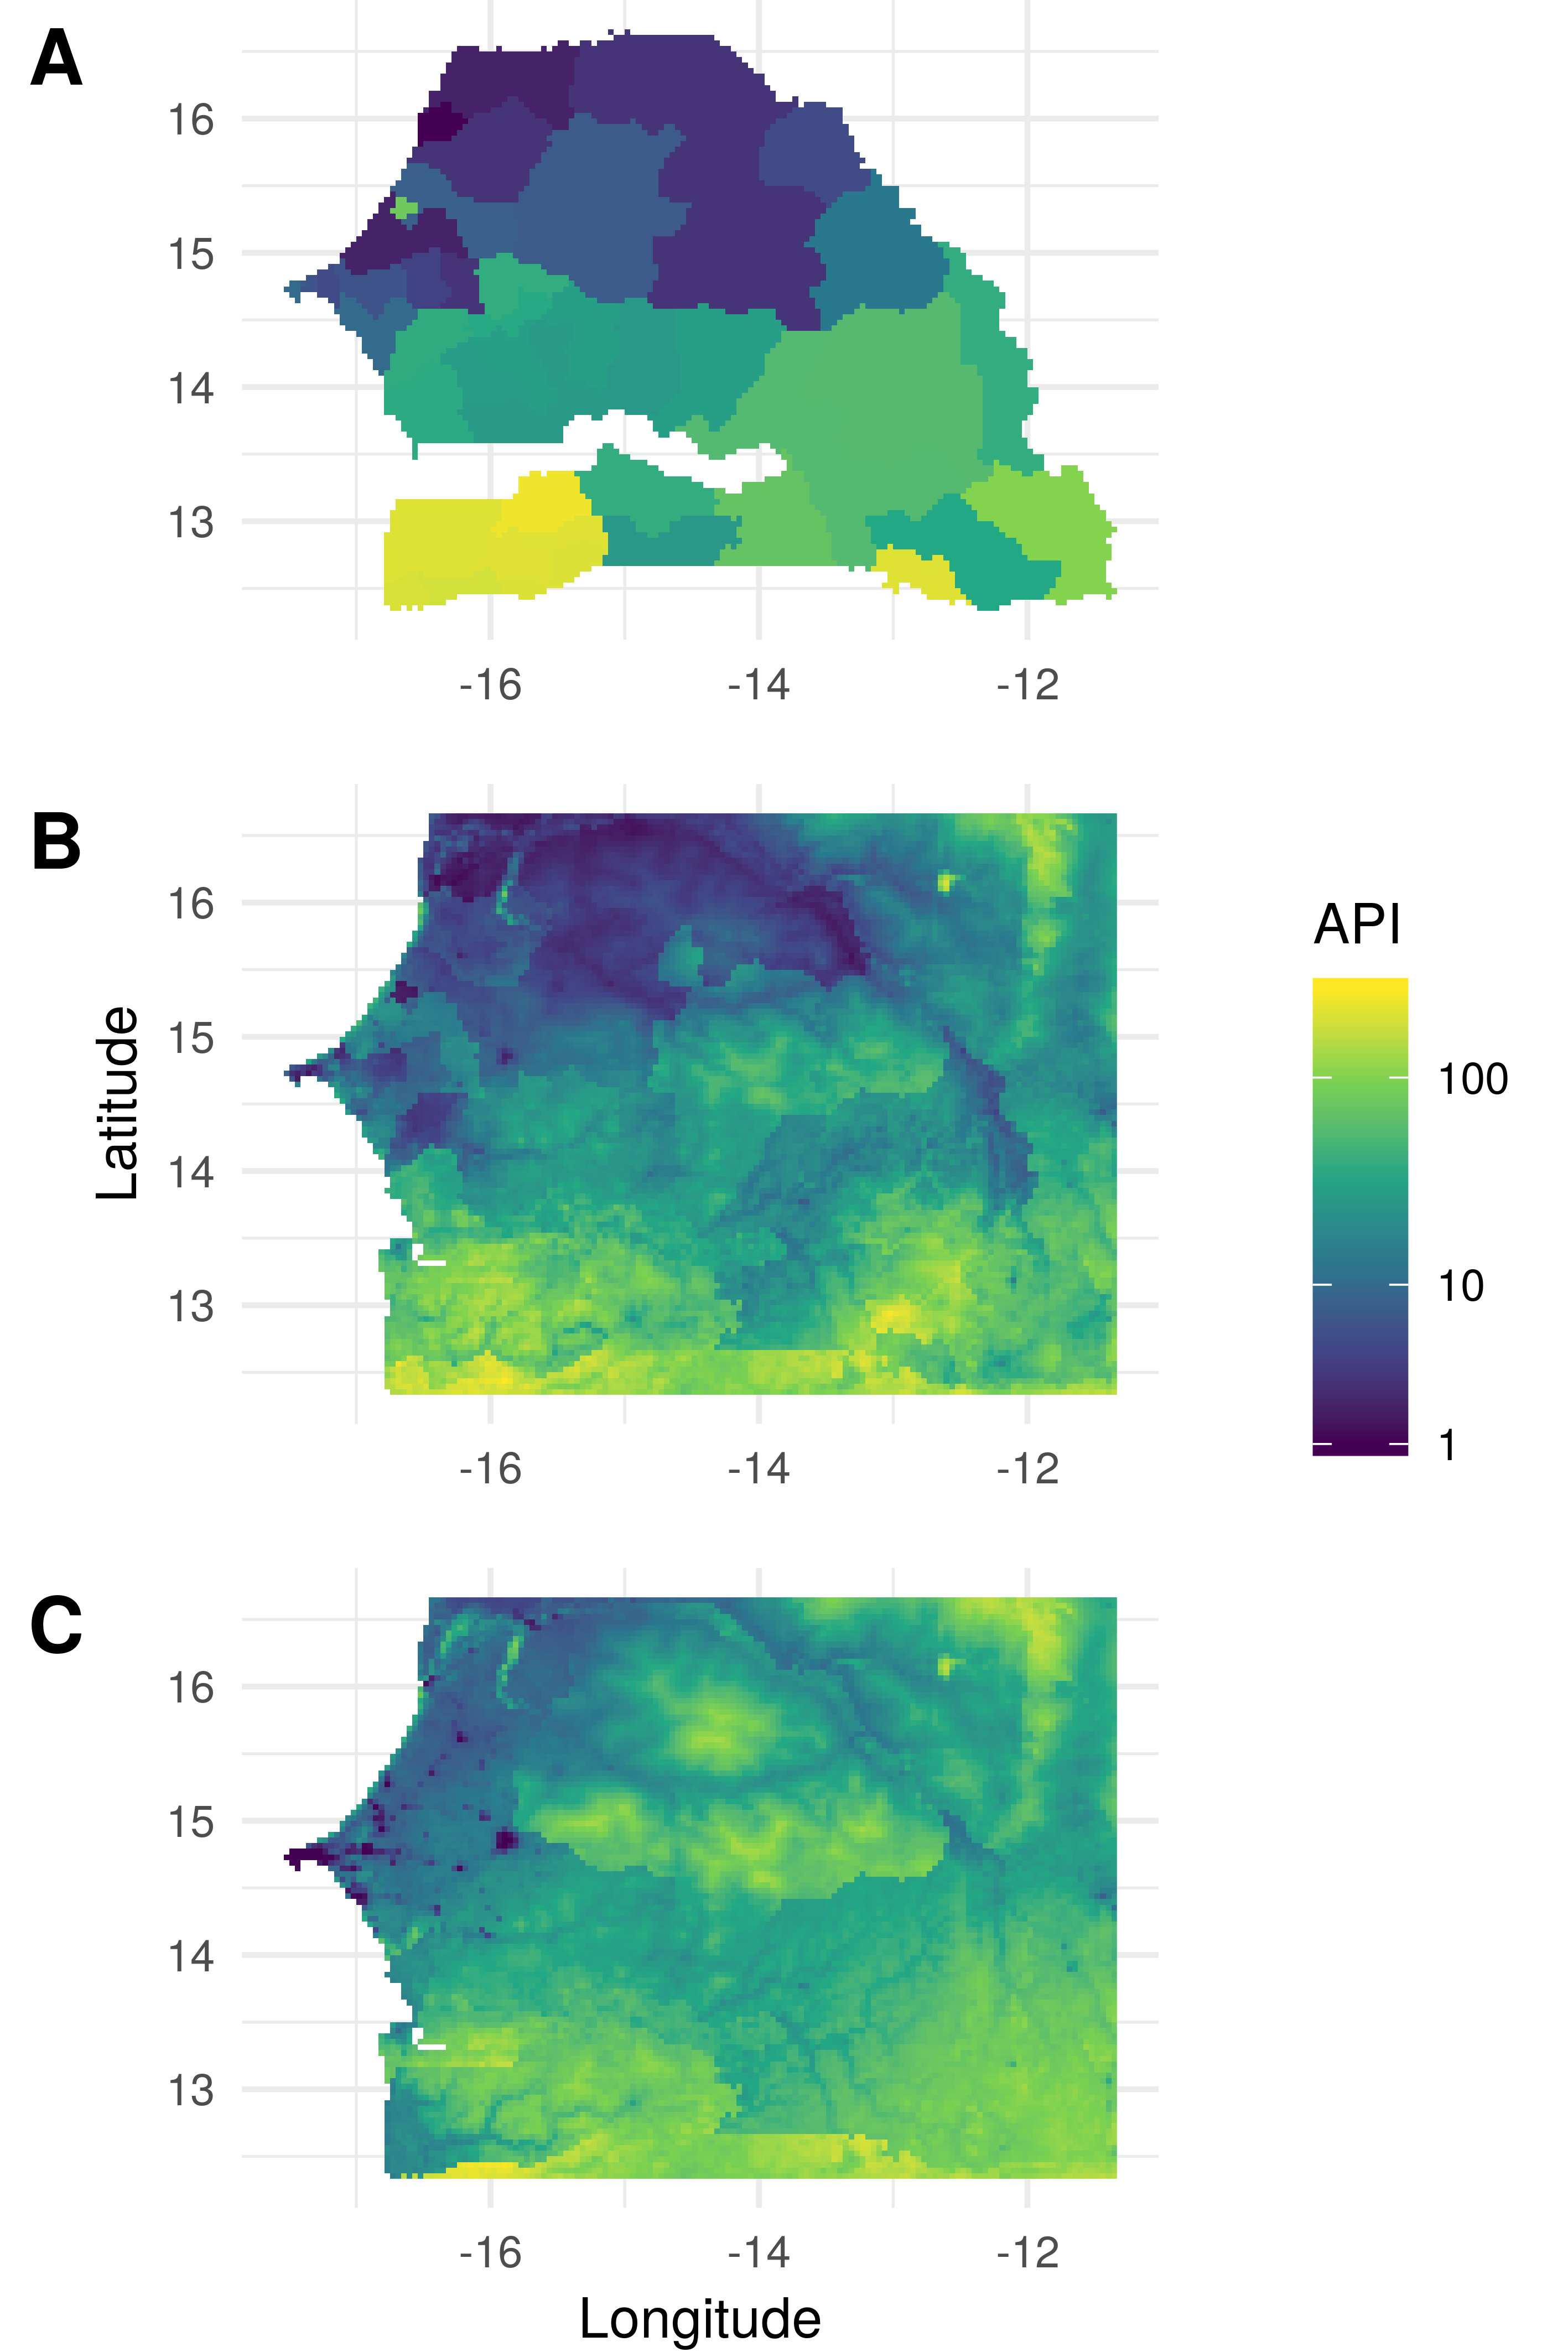
\includegraphics[width = 1.1\textwidth]{figures/sen_both_cv12_preds.png}}
\caption{\label{predobsmapsen}
Reported incidence data and modelled incidence maps for Senegal. 
The national boundary of Senegal is shown in grey and missing data is left white.
The adjusted input aggregated data is plotted in Panel A, while Panel B maps the predictions of the prevalence Gaussian Process model for for spatially cross-validated out-of-sample polygons and Panel C maps the predicted incidence from the joint model.
}

\end{figure}



\begin{figure}
% to be removed before submission
\makebox{\includegraphics[width = 1.1\textwidth]{figures/mdg_both_cv12_preds.png}}
\caption{\label{predobsmapmdg}
Reported incidence data and modelled incidence maps for Madagascar. 
The adjusted input aggregated data is plotted in Panel A, while Panel B maps the predictions of the prevalence Gaussian Process model for for spatially cross-validated out-of-sample polygons and Panel C maps the predicted incidence from the joint model.
}

\end{figure}



\begin{figure}[h!]
% to be removed before submission
\makebox{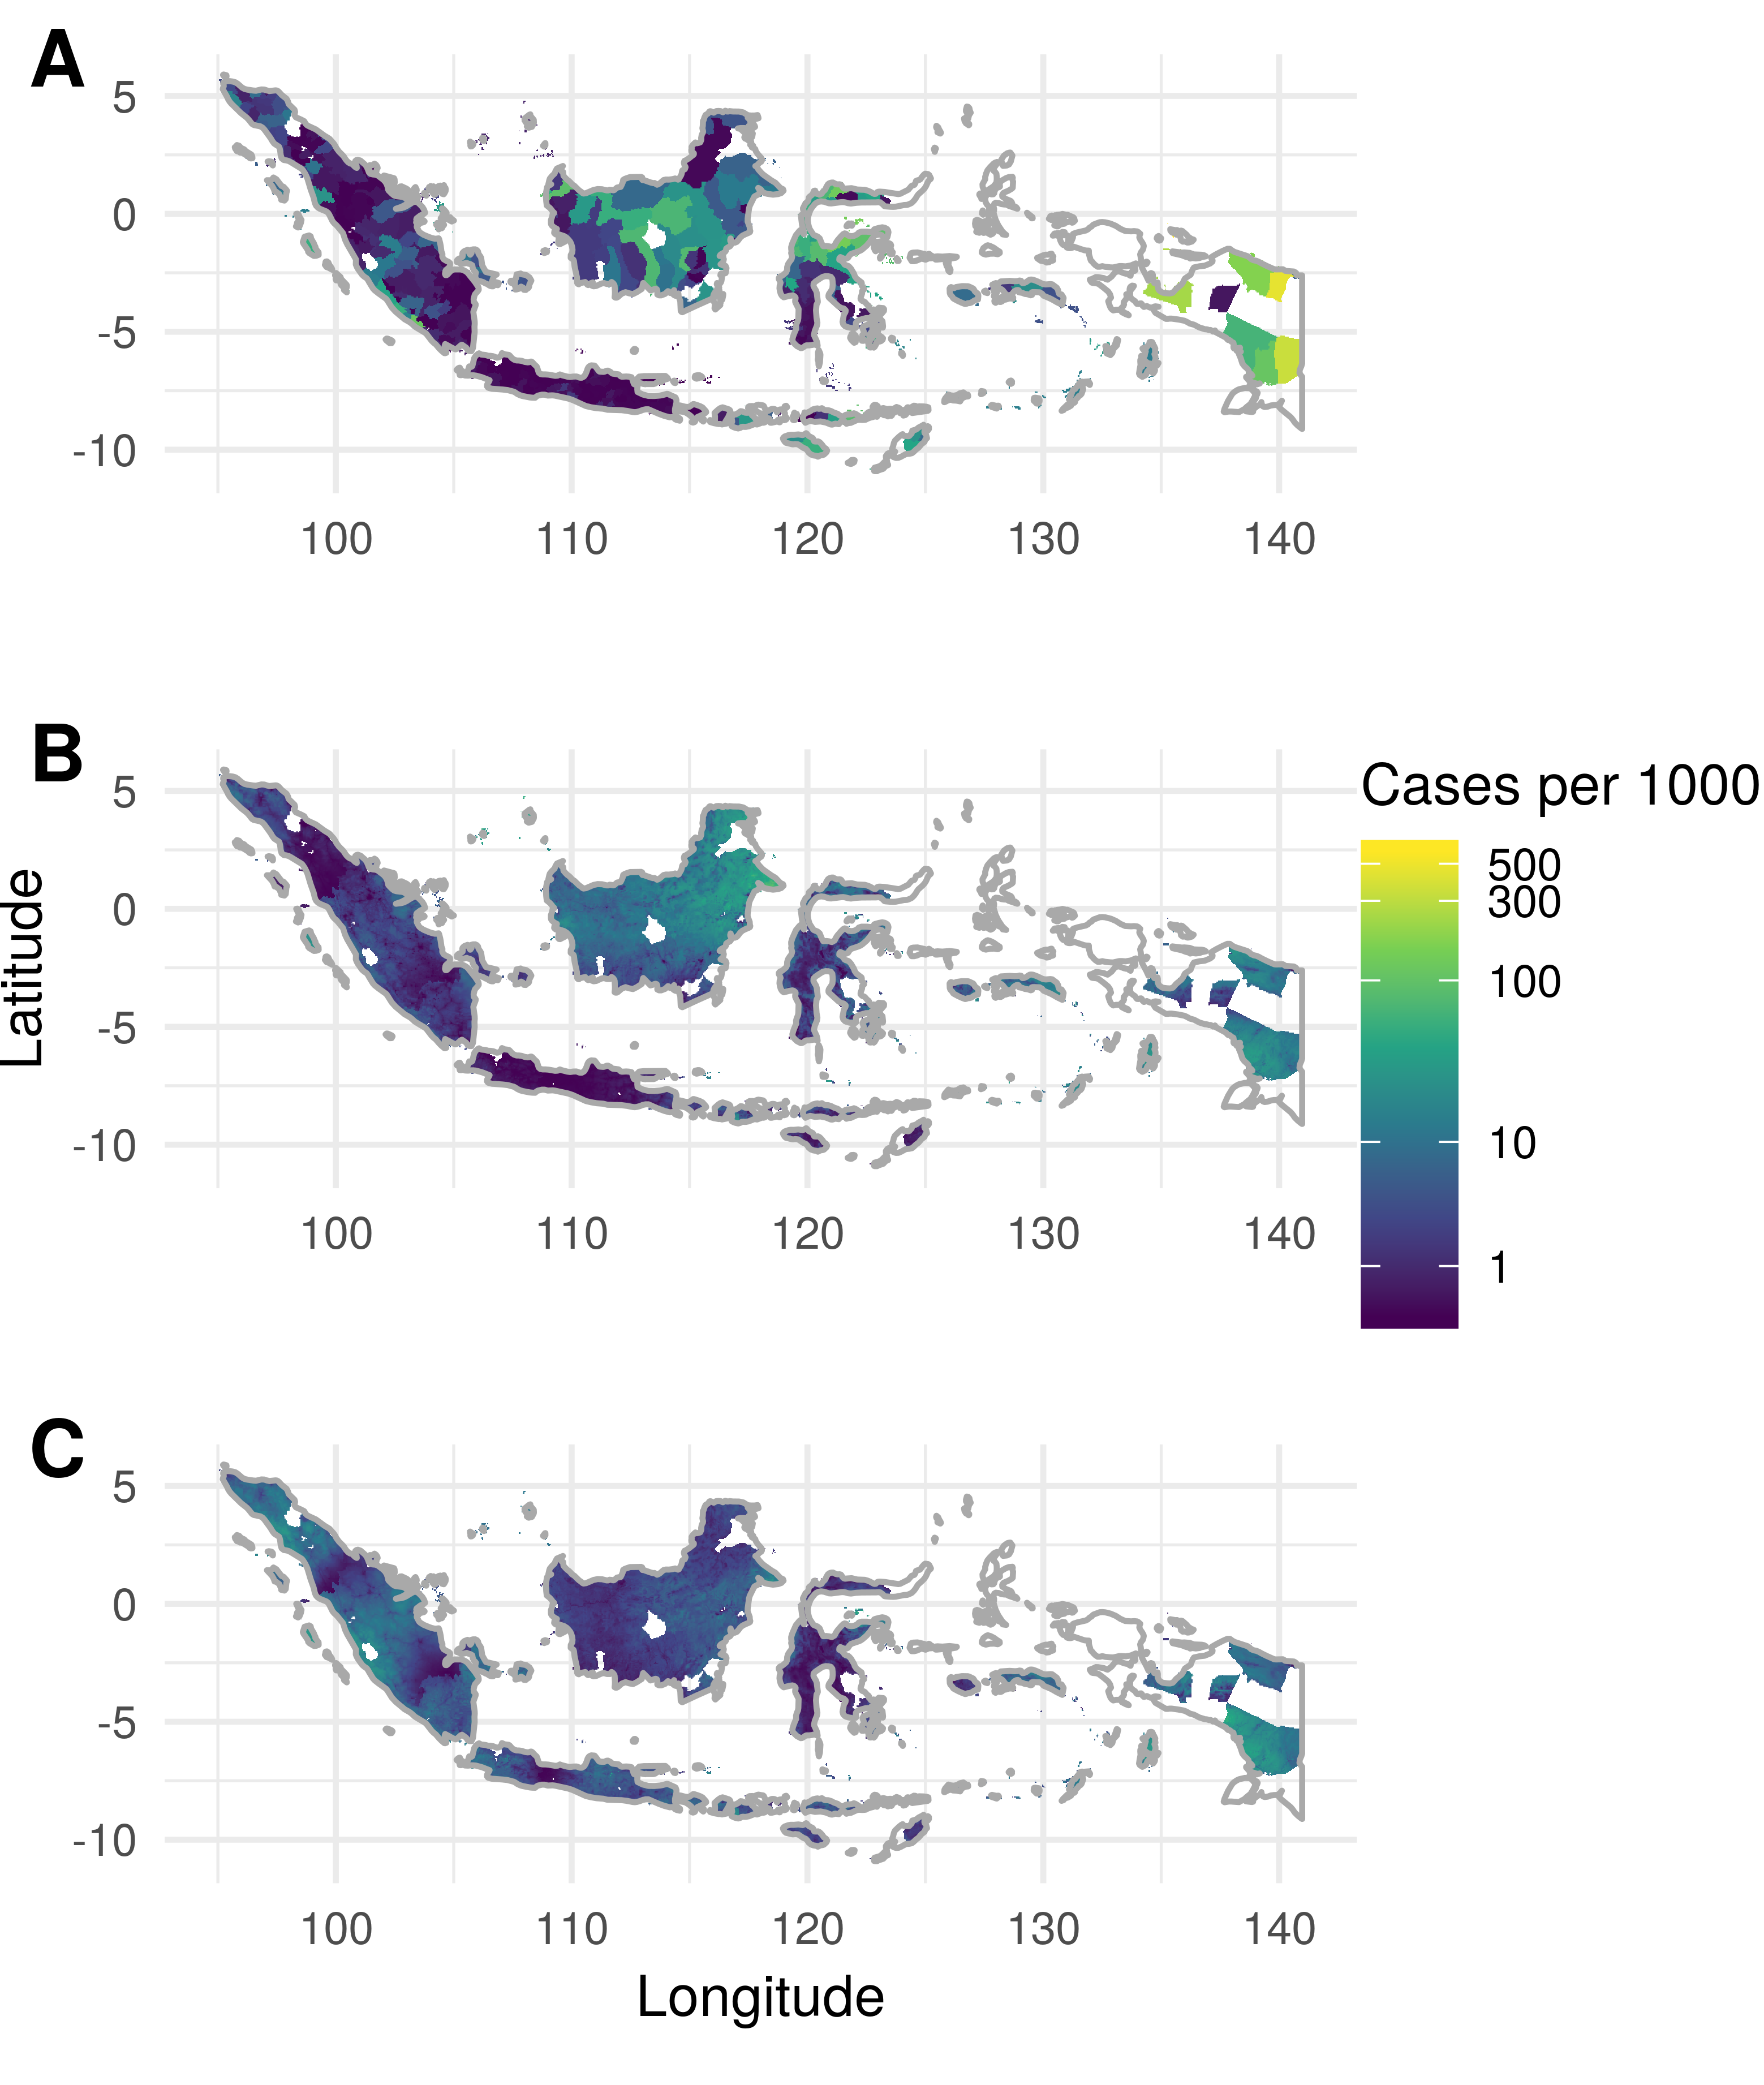
\includegraphics[width = 0.8\textwidth]{figures/idn_both_cv12_preds.png}}
\caption{\label{predobsmapidn}
Reported incidence data and modelled incidence maps for Indonesia. 
The national boundary of Indonesia is shown in grey and missing data is left white.
The adjusted input aggregated data is plotted in Panel A, while Panel B maps the predictions of the prevalence Gaussian Process model for for spatially cross-validated out-of-sample polygons and Panel C maps the predicted incidence from the joint model.
}
\end{figure}



\subsection*{Baseline Disaggregation Model}

Values at the aggregated, polygon (or areal) level are given the subscript $A$ while pixel or point level variables are indexed with $P$.
The polygon incidence case count data, $\mathrm{Count}_A$ is given a Poisson likelihood
$$\mathrm{Count}_A \sim \operatorname{Poisson}(\mathrm{Inc}_A\mathrm{pop}_A)$$
where $\mathrm{Inc}_A$ is the estimated polygon incidence rate and $\mathrm{pop_A}$ is the population at risk within that admin unit polygon (as apposed to the true health-centre catchment area).


Incidence rate is linked to latent pixel-level incidence ($\mathrm{Inc}_P$), prevalence ($\mathrm{Prev}_P$) and predictor variables by the following system of equations.
$$\mathrm{Inc}_A = \frac{ \sum_{P \in A}\mathrm{Inc}_P \mathrm{pop}_P}{\sum_{P \in A}\mathrm{pop}_P} $$
Here, $P \in A$ denotes that the summation is over the pixels in polygon $A$. 
Incidence is related to prevalence by
$$\mathrm{Inc}_P = \mathrm{PrevInc}(\mathrm{Prev}_P).$$
Here $\mathrm{PrevInc}$ is a function from a previously fitted model \citep{cameron2015defining}. 
$$\mathrm{PrevInc}: f\left(\mathrm{Prev}_P\right) = 2.6\cdot\mathrm{Prev}_P - 3.6\cdot{(\mathrm{Prev}_P)}^2 + 1.6\cdot{(\mathrm{Prev}_P)}^3.$$
The linear predictor of the model, $\eta_P$, is related to the latent prevalence scale by a typical logit link function.
$$\mathrm{Prev}_P = \operatorname{logit}^{-1}(\eta_P)$$
The baseline model is described in terms of prevalence as well as incidence, despite including no prevalence data, so that any differences in predictive ability compared to the full joint model are not simply due to the changed link function.
Furthermore, the form of this set of link functions means we calculated predictions of prevalence and incidence simultaneously whether both data types or just one were used which can be useful in applied settings.


The linear predictor is composed of an intercept, $b_0$, covariates, $X_P$, and a vector of regression coefficients $\boldsymbol\beta$.
We also include a spatial, Gaussian random field, $u_P(\rho, \sigma_u)$ and a polygon-level iid random effect, $ v_A(\sigma_v)$.
$$\eta_P = \beta_0 + \boldsymbol\beta X_P  + u_P(\rho, \sigma_u) + v_A(\sigma_v) $$
The Gaussian spatial effect $u_P(\rho, \sigma_u)$ has a Mat\'ern covariance function and two hyper parameters: $\rho$, the nominal range on the longitude-latitude scale (beyond which correlation is $< 0.1$) and $\sigma_u$, the marginal standard deviation.
The iid random effect, $v_A \sim \operatorname{Normal}(\mu = 0, \sigma = \sigma_v)$,  was grouped by polygon, with all pixels within polygon $A$ being grouped together (all subsequent normal distributions are also parameterised in terms of the standard deviation).
Internally, this effect is parameterised as the log of the precision, $\omega_v = \log(\tau_v) = \log(\frac{1}{{\sigma_v}^2})$ to improve numeric stability.
This random effect modelled both missing covariates and extra-Poisson sampling error.


Finally, we complete the model by setting priors on the parameters $\beta_0, \boldsymbol\beta, \rho, \sigma_u$ and $\sigma_v$.
The intercept was given a wide prior, $b_0 \sim \operatorname{Normal}(-2, 4)$, with a mean relating to a prevalence of 0.12 as we know \emph{a priori} that these countries have low or medium levels of malaria transmission.
We set independent, regularising priors on the regression coefficients $\beta_i \sim \operatorname{Normal}(0, 0.04)$. 
Given the standardised covariates, an intercept of -3 and a regression coefficient from the 95\% interquartile range of this distribution, each covariate would be able to predict prevalences between 0.004 and 0.27. 
This prior encodes our belief that the full range of malaria transmission can not be explained by a single covariate and our desire to regularise the model.
This regularisation is particularly important given the small number of administrative units in Senegal (n = 46) and Madagascar (n = 110).

We assigned $\rho$ and $\sigma_u$ a joint penalised complexity prior \citep{fuglstad2018constructing} such that $P(\rho < \zeta) = 0.00001$ and $P(\sigma_u > \xi) = 0.00001$.
We used different $\zeta$  and $\xi$ values for each country: Indonesia $\zeta = 3, \xi = 1$, Senegal $\zeta = 1, \xi = 0.5$ and Madagascar $\zeta = 1, \xi = 1$.
We believe that a large proportion of the variance of malaria prevalence and incidence cannot be explained by a linear combination of the covariates selected at the scale of individual countries \citep{bhatt2017improved}, so we set this prior such that the random field could explain most of the range of the data.
As Senegal has a lower range of incidences in the data we set $\xi$ to a smaller value for this country.
Plots of this prior are shown in Figure~S4 and S5.

We assigned $\sigma_v$ a penalised complexity prior \citep{simpson2017penalising} such that $P(\sigma_v > 0.05) = 0.0000001$.
This gives a 95\% prior credible interval of $7.8\times 10^{-5}$ -- $1.1\times 10^{-2}$.
This was based on a comparison of the variance of Poisson random variables, with rates given by the number of cases observed, and an separately derived upper and lower bound for the case counts using the approach defined by Cibulskis and colleagues \citep{cibulskis2011worldwide}.
We found that an iid effect with a standard deviation of 0.05 was able to account for the discrepancy between the assumed Poisson error and the separately derived measurement error.

The models were implemented and fitted in R \citep{R} using Template Model Builder \citep{TMB} which allows a Laplace approximation of the posterior to be calculated.
We note that R-INLA \citep{INLA} can be used to fit disaggregation models but only when a linear link function is being used \citep{wilson2017pointless}.
The hyperparameters are fitted using empirical Bayes whereby the hyperparameters are learned from the data but are treated as point estimates rather than using the full posterior of the hyperparameters.
We further note that MCMC, even using efficient samplers, is prohibitively slow for these sorts of models \citep{nandi2020disaggregation}. 


%\begin{figure}[t!]
%% to be removed before submission
%\centering
%
%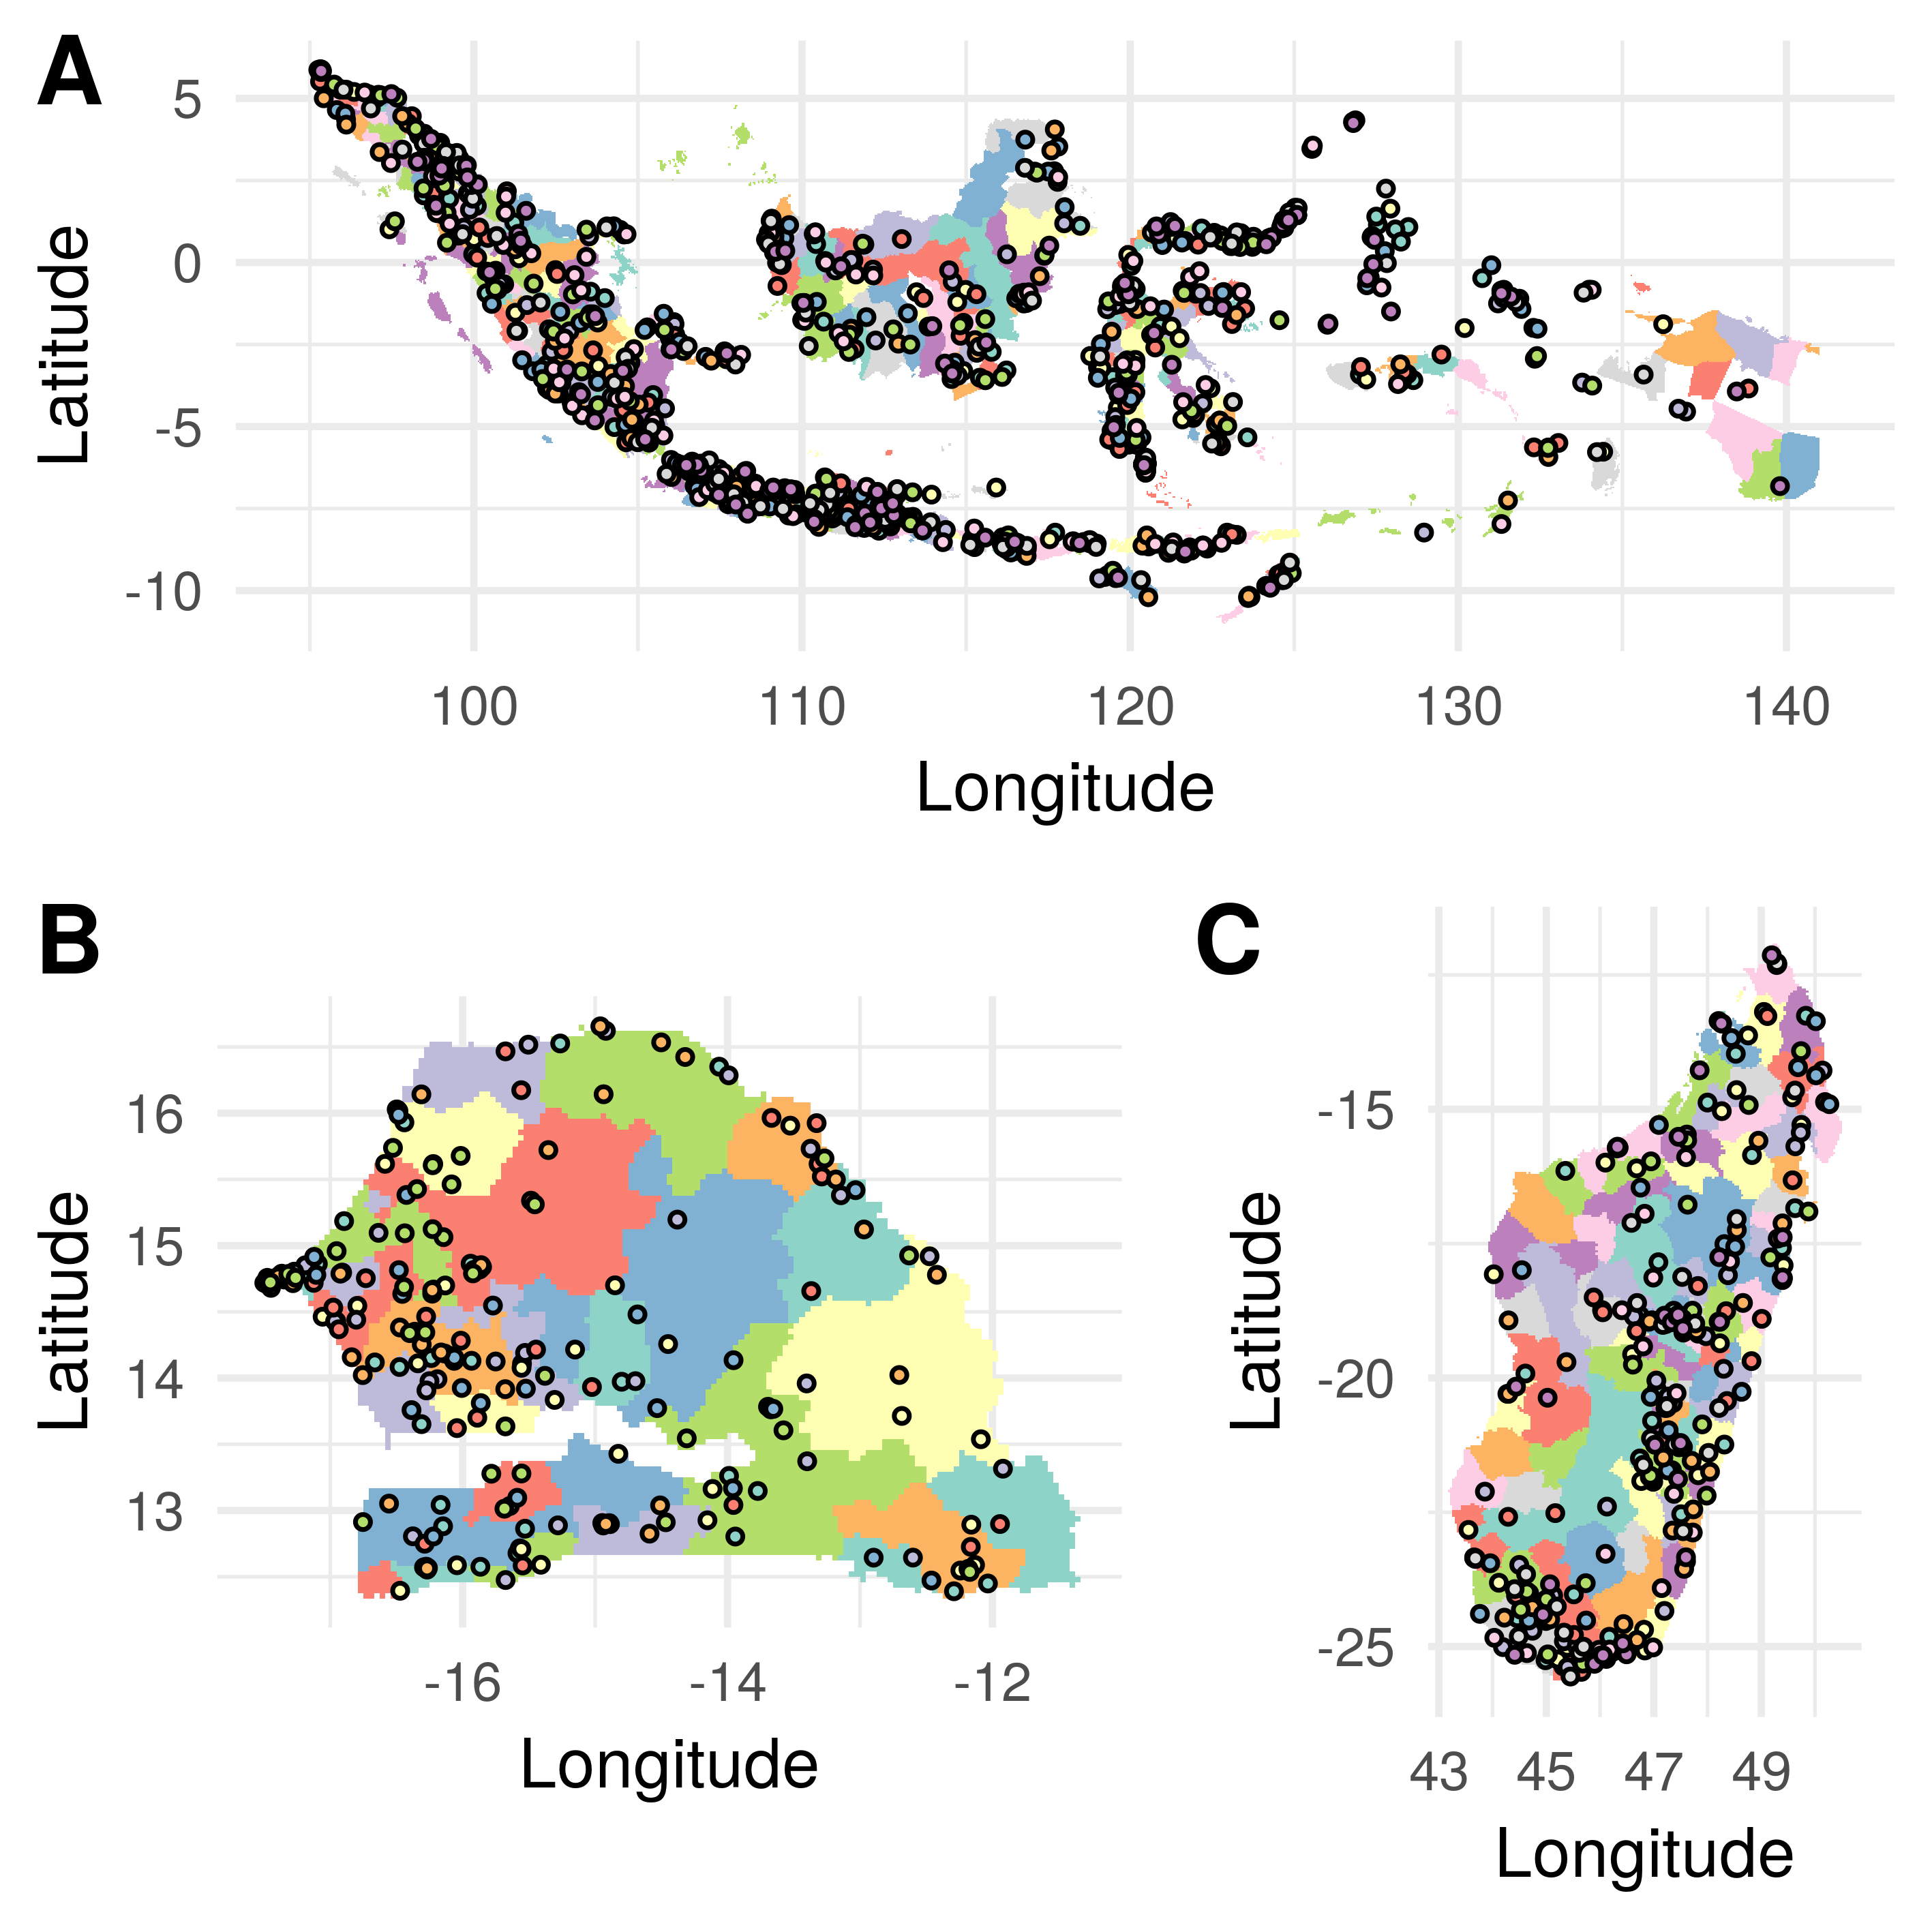
\includegraphics[width = 0.9\textwidth]{figures/random_crossvalidation_full.png} %\caption{Indonesia random crossvalidation} 
%
%\caption{{\bf Random cross-validation scheme for Indonesia, Senegal and Madagascar.} The fold for both aggregated incidence data and prevalence point data is shown.}
%\label{fig:cv_random}
%\end{figure}
%
%
%\begin{figure}[!t]
%% to be removed before submission
%\centering
%
%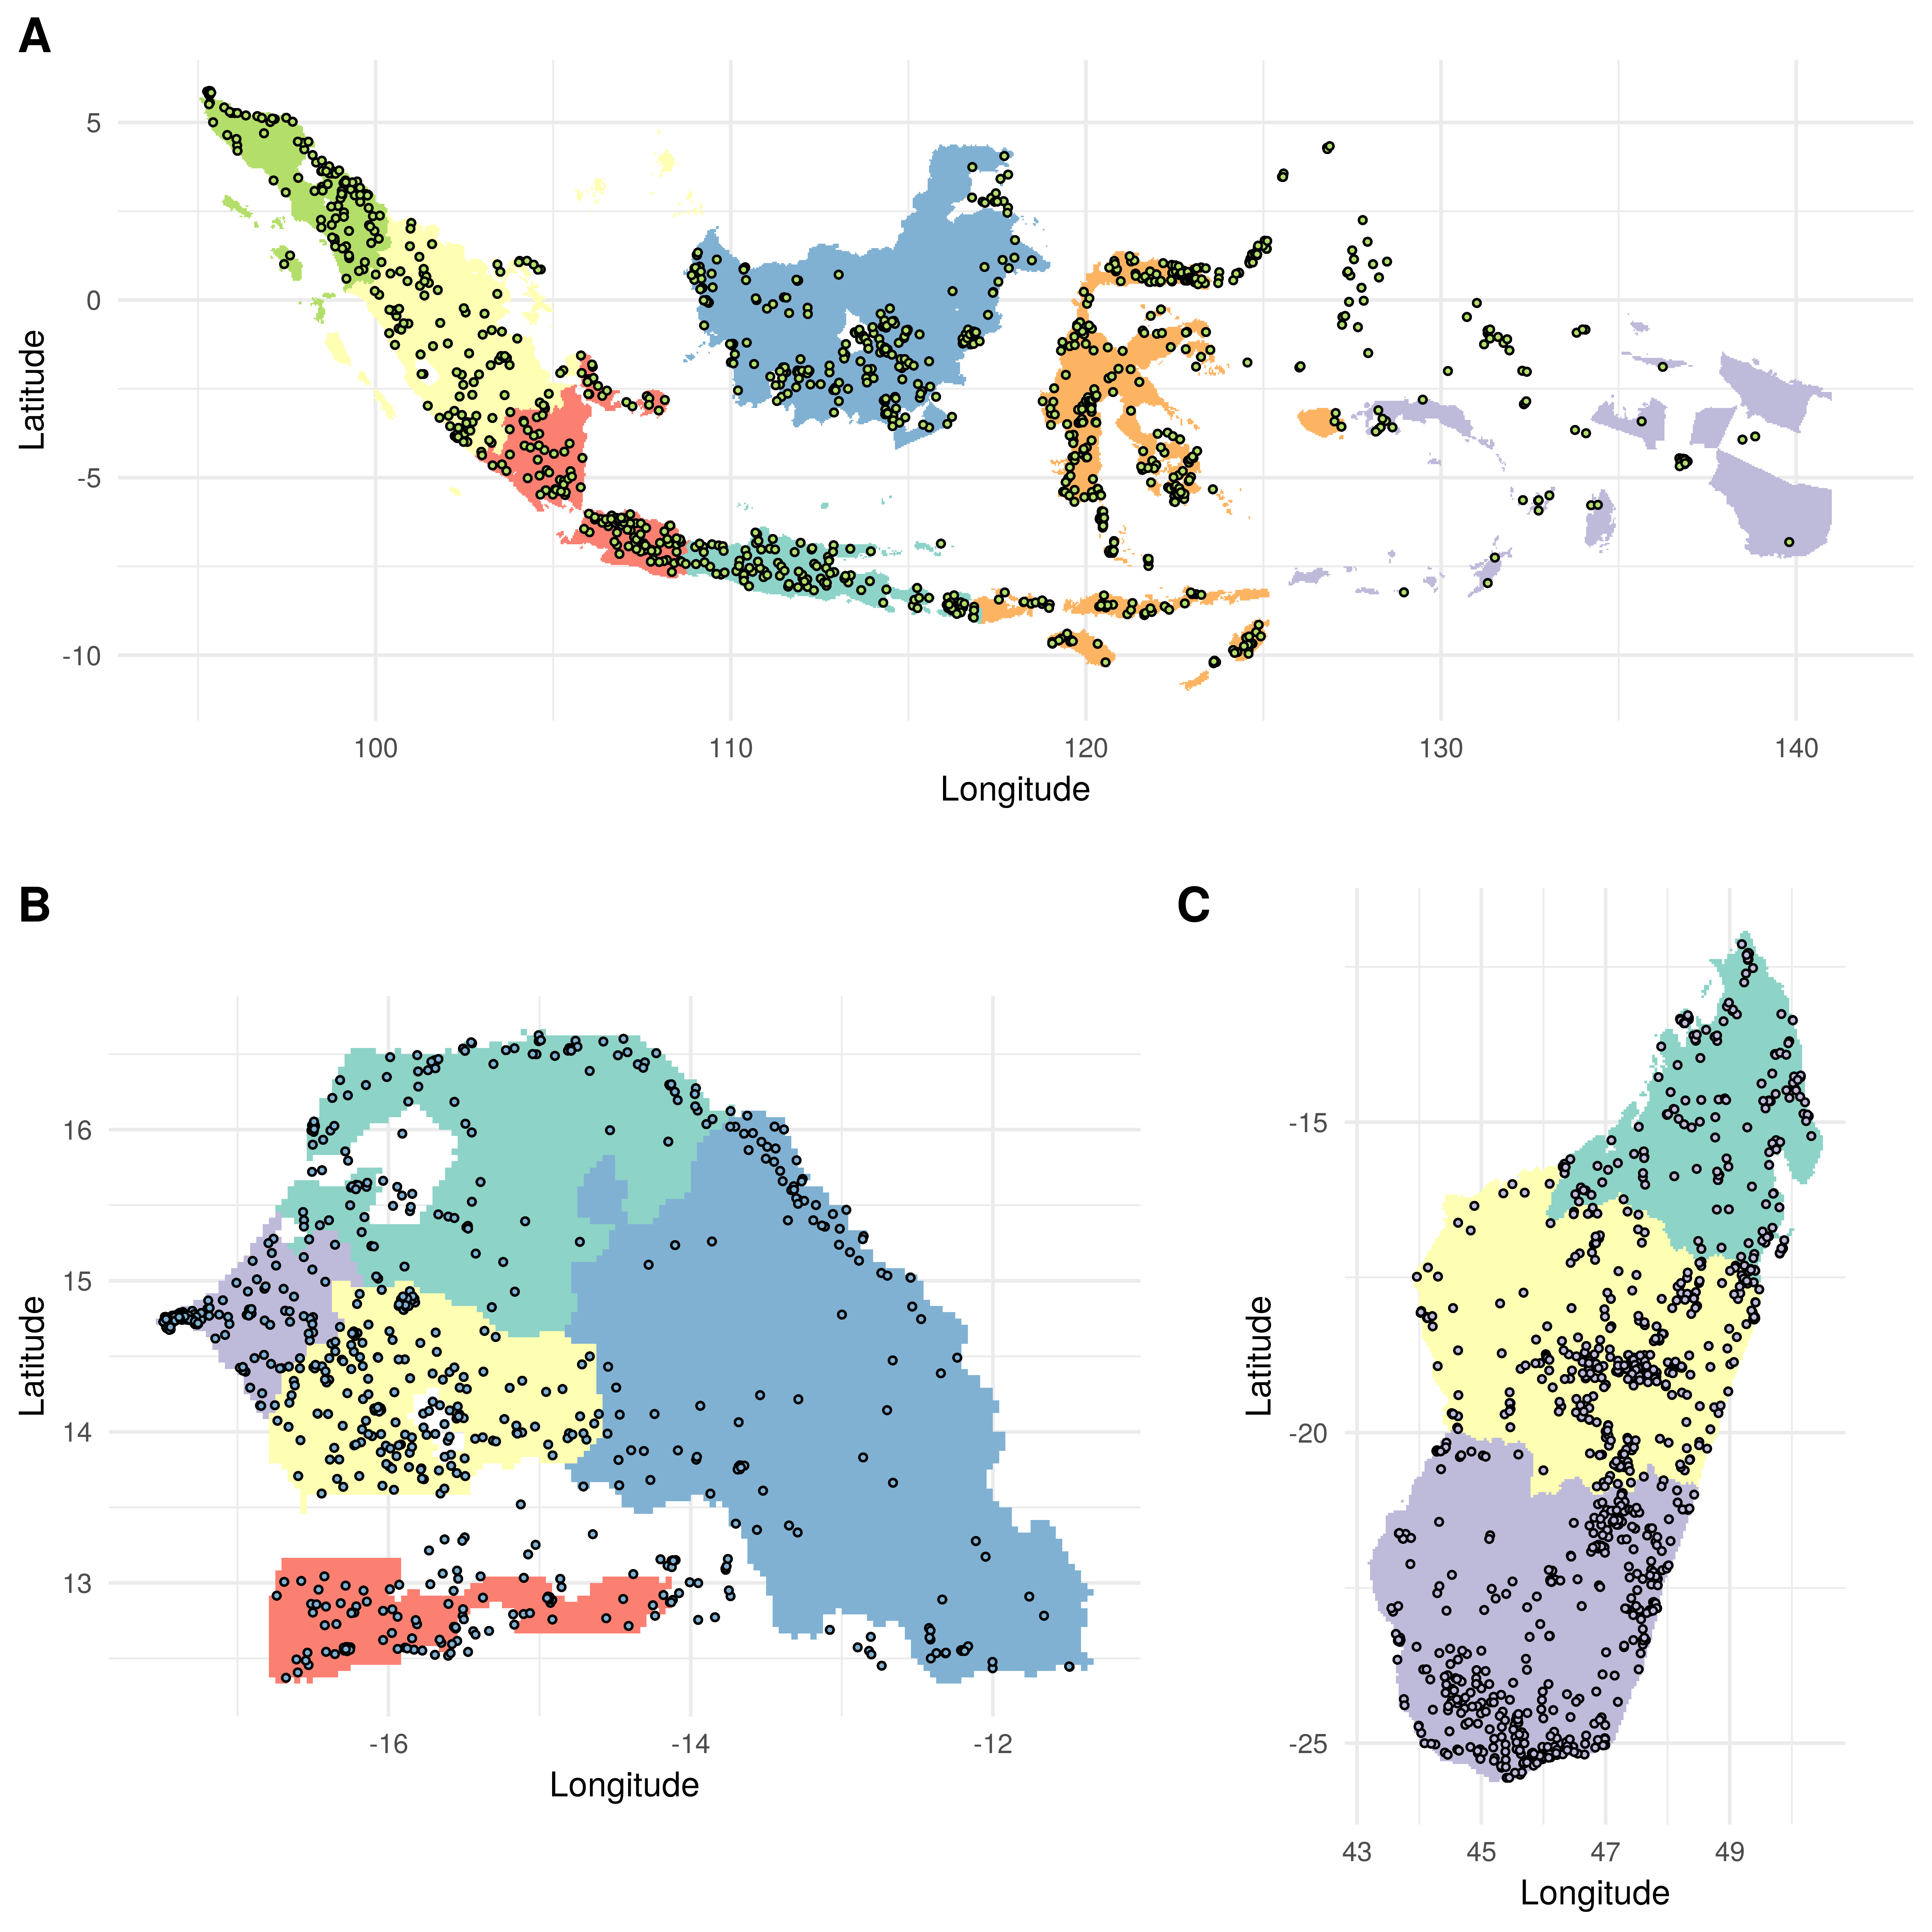
\includegraphics[width = 0.9\textwidth]{figures/spatial_crossvalidation_full.png} %\caption{Indonesia random crossvalidation} 
%
%\caption{{\bf Spatial cross-validation scheme for Indonesia, Senegal and Madagascar.} The fold for both aggregated incidence data and prevalence point data is shown.}
%\label{fig:cv_spatial}
%\end{figure}
%

\subsection*{Prevalence Gaussian process covariate model}

The prevalence Gaussian Process model (henceforth the prevalence GP model) is the same as the baseline disaggregation model except that it has one extra covariate.
This covariate is created by fitting a Gaussian random field to the prevalence survey data.
For each country we fitted a model with a binomial likelihood.
$$z_P \sim \operatorname{Binomial}(\mathrm{Prev}_P, n_P) $$
Here $\mathrm{Prev}_P$ is the estimated prevalence and $n_P$ is the observed survey sample size. 
The model only depended on a Gaussian random field having no covariates or an intercept.
$$\mathrm{Prev}_P = \operatorname{logit}^{-1}(u_P(\rho, \sigma_u))$$
We used the same hyperpriors for $\rho$ and $\sigma_u$ as above. 
These models were fitted using R-INLA \citep{INLA}.
To be in the correct scale for the dissagregation model, the inverse logit of the predicted Gaussian field (i.e. the linear predictor of the model) was used as the additional covariate.

\subsection*{Full joint model}

The final model is a joint-likelihood model with separate likelihoods for prevalence point-surveys and polygon incidence data.
The polygon data are assigned a Poisson likelihood as before.
Additionally, the point-survey data, with positive cases $z_b$, are given a binomial likelihood
$$z_P \sim \operatorname{Binomial}(\mathrm{Prev}_P, n_P) $$
where $\mathrm{Prev}_P$ is the estimated prevalence and $n_P$ is the observed survey sample size. 
As this model has both prevalence and incidence data we add a parameter $\alpha$ that modifies the relationship between the two.
$$\mathrm{Inc}_P = \exp(\alpha)\mathrm{PrevInc}(\mathrm{Prev}_P).$$
The only further additions to the baseline model are in the linear predictor which becomes 
$$\eta_P = \beta_0 + \mathbf{1}_\mathrm{Prev}\beta_\mathrm{Prev} +  \boldsymbol\beta X_P  + u_P(\rho, \sigma_u) + v_A(\sigma_v) + w_P(\sigma_w).$$
As well as the global intercept, $\beta_0$, this model has a prevalence survey specific intercept $\beta_\mathrm{Prev}$ where the indicator function, $\mathbf{1}_\mathrm{Prev}$, denotes that this term is zero except when a prevalence point-survey is being considered.
The iid random effect, $v_A \sim \operatorname{Norm}(0, \sigma_v)$, was again grouped by polygon, with all pixels and point-surveys within polygon $A$ being in the same group as polygon $A$.
The second iid random effect, $w_P \sim \operatorname{Normal}(0, \sigma_w)$, was applied to each point-survey.
To improve numeric stability this effect is also parameterised internally as the log of the precision, $\omega_w = \log(\tau_w) = \log(\frac{1}{{\sigma_w}^2})$.
This effect modelled extra-binomial sampling noise.
As such, this random effect is not included in the predicted uncertainty in the incidence or prevalence layers.


We assigned $\sigma_w$ a penalised complexity prior such that $P(\sigma_w > \phi) = 0.0000001$. 
This was chosen by finding the maximum difference in prevalence between point-surveys (with a sample size greater than 500 individuals) within the same raster pixel.
The differences between points within the same pixel can only be accounted for by the binomial error and this iid effect.
Given that the error on a prevalence estimate with sample size greater than 500 is quite small, the iid effect needs to be able to explain this difference.
In Senegal and Madagascar this value was relatively small so we set $\phi = 0.05$. 
In Indonesia however, there was a high density of prevalence surveys and heterogeneity in estimated prevalence within single pixels.
Therefore we set $\phi = 0.3$.

The PrevInc relationship was fitted to the best available data (matched prevalence and incidence studies both at point level) and this dataset.
Therefore we have some \emph{a priori} confidence in it and from a regularisation standpoint would not wish it to be easily overridden by the data used in these models which are mismatched in spatial scale.
Therefore, our prior belief is that $\exp(\alpha)$ is close to one (i.e.\thinspace the relationship remains unchanged) and therefore that $\alpha$ is close to zero.
We set our prior as $\alpha \sim \operatorname{Normal}(0, 0.001)$.


\subsection*{Experiments}

To compare the three models we used two cross-validation schemes. 
In the first (random), the incidence data was split into ten cross-validation folds while all the prevalence data was used in each case (Figure~S1). 
%This cross-validation scheme directly addresses the question of whethe
In the second validation scheme, the incidence data was split into spatial cross-validation folds, using k means clustering on polygon centroids, while again all prevalence points were used in all folds (Figure~S2).
The number of folds was seven for Indonesia, five for Senegal and three for Madagascar.
The number of folds was chosen based on the geographical sizes of the countries.
This scheme tests specifically whether the joint model can improve predictions by increasing geographic data coverage.
In each case we tested whether the differences between the new models and the baseline model was greater than expected  by chance using a paired Wilcox test.
%This situation is particularly common in continental scale models where some countries will have large DHS style surveys but little incidence data.



\begin{table}
\caption{\label{table1}Summary of out-of-sample accuracy for all cross-validation experiments. 
Mean absolute error of predicted incidence rate against out-of-sample observed data for three countries. 
Results that are significantly better or worse than the baseline (at the 95\% significance level) are indicated with a dagger or asterisk respectively.
}
\centering
\fbox{%
\begin{tabular}{*{5}{l}}
{\bf Cross-validation} & {\bf Country}  & {\bf Baseline} & {\bf Prev GP} & {\bf Joint} \\
\hline
Random & Indonesia  & 13.95 &  14.09 &  13.79\\
& Senegal  & 12.41 &  12.37 &  13.07\\
& Madagascar  & 39.06 & 35.82 &  39.01\vspace{3mm}\\
Spatial & Indonesia & 14.77 & 14.77 &  16.46$\ast$\\
& Senegal  & 13.09 &   12.21 &  15.15$\ast$\\
& Madagascar & 67.73 &  50.38\dag &  44.05\dag\\
\end{tabular}}
\end{table}


We considered the ability of the model to predict polygon incidence to be our main objective and our performance metric for this was mean absolute error (MAE).
As the models were fitted on data on different scales we found that observations and predictions were sometimes correlated but shifted from the one-one line (i.e. were biased) and therefore correlation metrics were misleading.
% Why not correlation
To assess how well the models were calibrated we considered coverage of the 80\% predictive credible intervals on the hold-out data.
Finally we compared the widths of the posterior distributions for the regression parameters (the $\beta_i$'s) and the hyperparameters for the random field ($\rho$ and $\sigma_u$).
For these comparisons we report the average of the standard deviations of the posteriors for each group of parameters across all the random cross-validation model fits.
The prevalence GP model has one more $\beta_i$ than the other two models that relates to the additional covariate created by fitting a Gaussian Process to prevalence data. 
We did not include this parameter when comparing the widths of the $\beta_i$ parameters.
%Finally, we fitted each model to the full data set and examine the parameter estimates for these models.


\subsection*{Sensitivity analysis}

We ran sensitivity analyses for particular aspects of the model and prior specification.
We limited our sensitivity analysis to Madagascar and ran random cross-validation on the full joint model with a number of alterations.
We tested a weaker prior on $\alpha$, using $\alpha \sim \operatorname{Normal}(0, 1)$ instead of $\alpha \sim \operatorname{Normal}(0, 0.001)$.
We also examined the sensitivity of the model to the coefficient values used in the PrevInc function. 
We reran the cross-validation using five draws from a normal distribution, centred on the original parameter values, and with a standard deviation of 0.1.
Finally, we reran the cross-validation using weaker priors on the random effects but keeping the relative strengths of the iid and spatial random effects the same.
We used $P(\sigma_u > 1) = 0.01$ and $P(\sigma_v > 0.05) = 0.001$.




% Results and Discussion can be combined.
%%%%%%%%%%%%%%%%%%%%%%%%%%%%%%%%%%%%%%%%%%%%%%%%%%%%%%%%%%%%%%%%%%%%%%%%%%%%%%%%%%%%%%%%%%%%%%%%%%%%%
\section*{Results}
%%%%%%%%%%%%%%%%%%%%%%%%%%%%%%%%%%%%%%%%%%%%%%%%%%%%%%%%%%%%%%%%%%%%%%%%%%%%%%%%%%%%%%%%%%%%%%%%%%%%%

% Random cv

Under the random cross-validation scheme, there was no significant differences in model performance between models (Table \ref{table1}).
This lack of strong differences is highlighted by there being no clear differences in scatter plots of observed and predicted data across the three methods (Figure S3).
Under the spatial cross-validation scheme, the prevalence GP model performed significantly better than baseline in Madagascar and was not significantly different from baseline in Indonesia or Senegal (Table \ref{table1}).
The joint model performed significantly worse than baseline in Indonesia and in Senegal but was the best performing model in Madagascar.
Furthermore, notable differences can be seen in the scatter plots of observed and predicted values (Figure \ref{spatial2predobspolyfacet}).
In Indonesia it can be seen that the joint model is more strongly biased at low incidence values with many data points being overpredicted.
However, the joint model clearly performs better in Madagascar with the polygon-only model unable to predict high incidence observations accurately.
Out-of-sample predictions, under spatial cross validation, from the prevalence GP model and full joint model can be seen in Figures~\ref{predobsmapsen} -- \ref{predobsmapidn}.
%figure 5, 6. Spat and random cv. PR vs Poly columns, countries as rows, model as colour?


\begin{figure}
% to be removed before submission
\makebox{\includegraphics[width = 1.05\textwidth]{figures/spatialkeeppr_cv_poly_facet.pdf}}
\caption{\label{spatial2predobspolyfacet} 
Observed-predicted plots of modelled annual malaria incidence (cases per 1000) by country from the spatial cross-validation experiments for Indonesia (Panel A), Senegal (Panel B) and Madagascar (Panel C). 
Results from the baseline disaggregation model are shown in red, the prevalence GP model is shown in green while the joint model is shown in blue.
The one-one line is shown with a black line and a simple linear regression through the points is shown by a coloured line.
}

\end{figure}
% todo add country names to plots.


% Coverage results

All models seem to be fairly well calibrated (Table~\ref{table3}).
The proportion of out-of-sample incidence datapoints being within their 80\% credible intervals ranged between 0.51 and 0.88.
However, in most cases coverage was between 0.7 and 0.8 implying that the models were a little overconfident in their predictions.
There was no clear difference in calibration between the different models.

% Look at parameters

We can further investigate why the models performed as they did by examining the parameters estimated in the models fitted to all data (Tables~S1--S3).
Firstly we can compare the regression parameter for the prevalence GP covariate in the three countries noting that in Indonesia the prevalence GP model performed worse than baseline under random cross-validation and had equal performance to baseline under spatial cross-validation.
We see that the regression parameter for this covariate was small in Indonesia (mean = 0.06, sd = 0.12) but relatively large and positive in both Senegal (mean = 0.30, sd = 0.17) and Madagascar  (mean = 0.36, sd = 0.07).

In Madagascar the joint model performed the best in the spatial cross-validation scheme and better than the baseline in the random cross-validation scheme. 
Comparing the estimated parameters of the joint model between Madagascar and the other two countries therefore is useful.
The prevalence intercept, $\beta_p$, is large in the Senegal fit (mean = 1.36, sd = 0.13) but small in Indonesia (mean = 0.03, sd = 0.20) and Madagascar (mean = 0.07, sd = 0.10).
This implies there is a strong discrepency (given the prevalence to incidence model) between the prevalence and incidence data in Senegal.
Furthermore, the standard deviation of the prevalence point iid effect, $w_b(\sigma_w)$, is much larger in Indonesia (mean $\omega_w = -2.6$, sd $\omega_w = 0.09$ which corresponds to a mean of $\sigma_w$ of 13.46) than in Senegal (mean $\omega_w = -1.03$, sd $\omega_w = 0.13$ which corresponds to a mean of $\sigma_w$ of 2.80) or Madagascar (mean $\omega_w = -0.77$, sd $\omega_w = 0.11$ which corresponds to a mean of $\sigma_w$ of 2.16).
This implies there is a lot of noise in the prevalence data in Indonesia.

We set a strong prior on $\alpha$ being close to one, encoding our belief that the incidence prevalence relationship should be close to the previously fitted model.
The estimated value for $\alpha$ in all three countries is very close to one (Tables~S1--S3).
While this might be driven by the prior, this indicates that there is no strong evidence from the data that this relationship should be scaled differently by country.
The MAE for Madagascar does not change when run with a much weaker prior on this parameter.
However, the MAE for Madagascar varies quite a lot when adding random noise to the parameter values (MAE increases by between 0 and 5.7).
Changing the priors on the iid effect and the marginal standard deviation of the Gaussian random field did not alter predictive performance.

%\subsection{Parameter estimates}
% We can examine the parameters in the models fitted
% discuss beta for prev go
% discuss alpha 
% are other betas the same across models and countries.


%figure 3 and 4. data and predicted incidence maps. Indonesia and Senegal only. Fig 3 ind, fig 4 rand. Data, Rand, Spatial for best model? Joint model?

%\begin{figure}
% to be removed before submission
%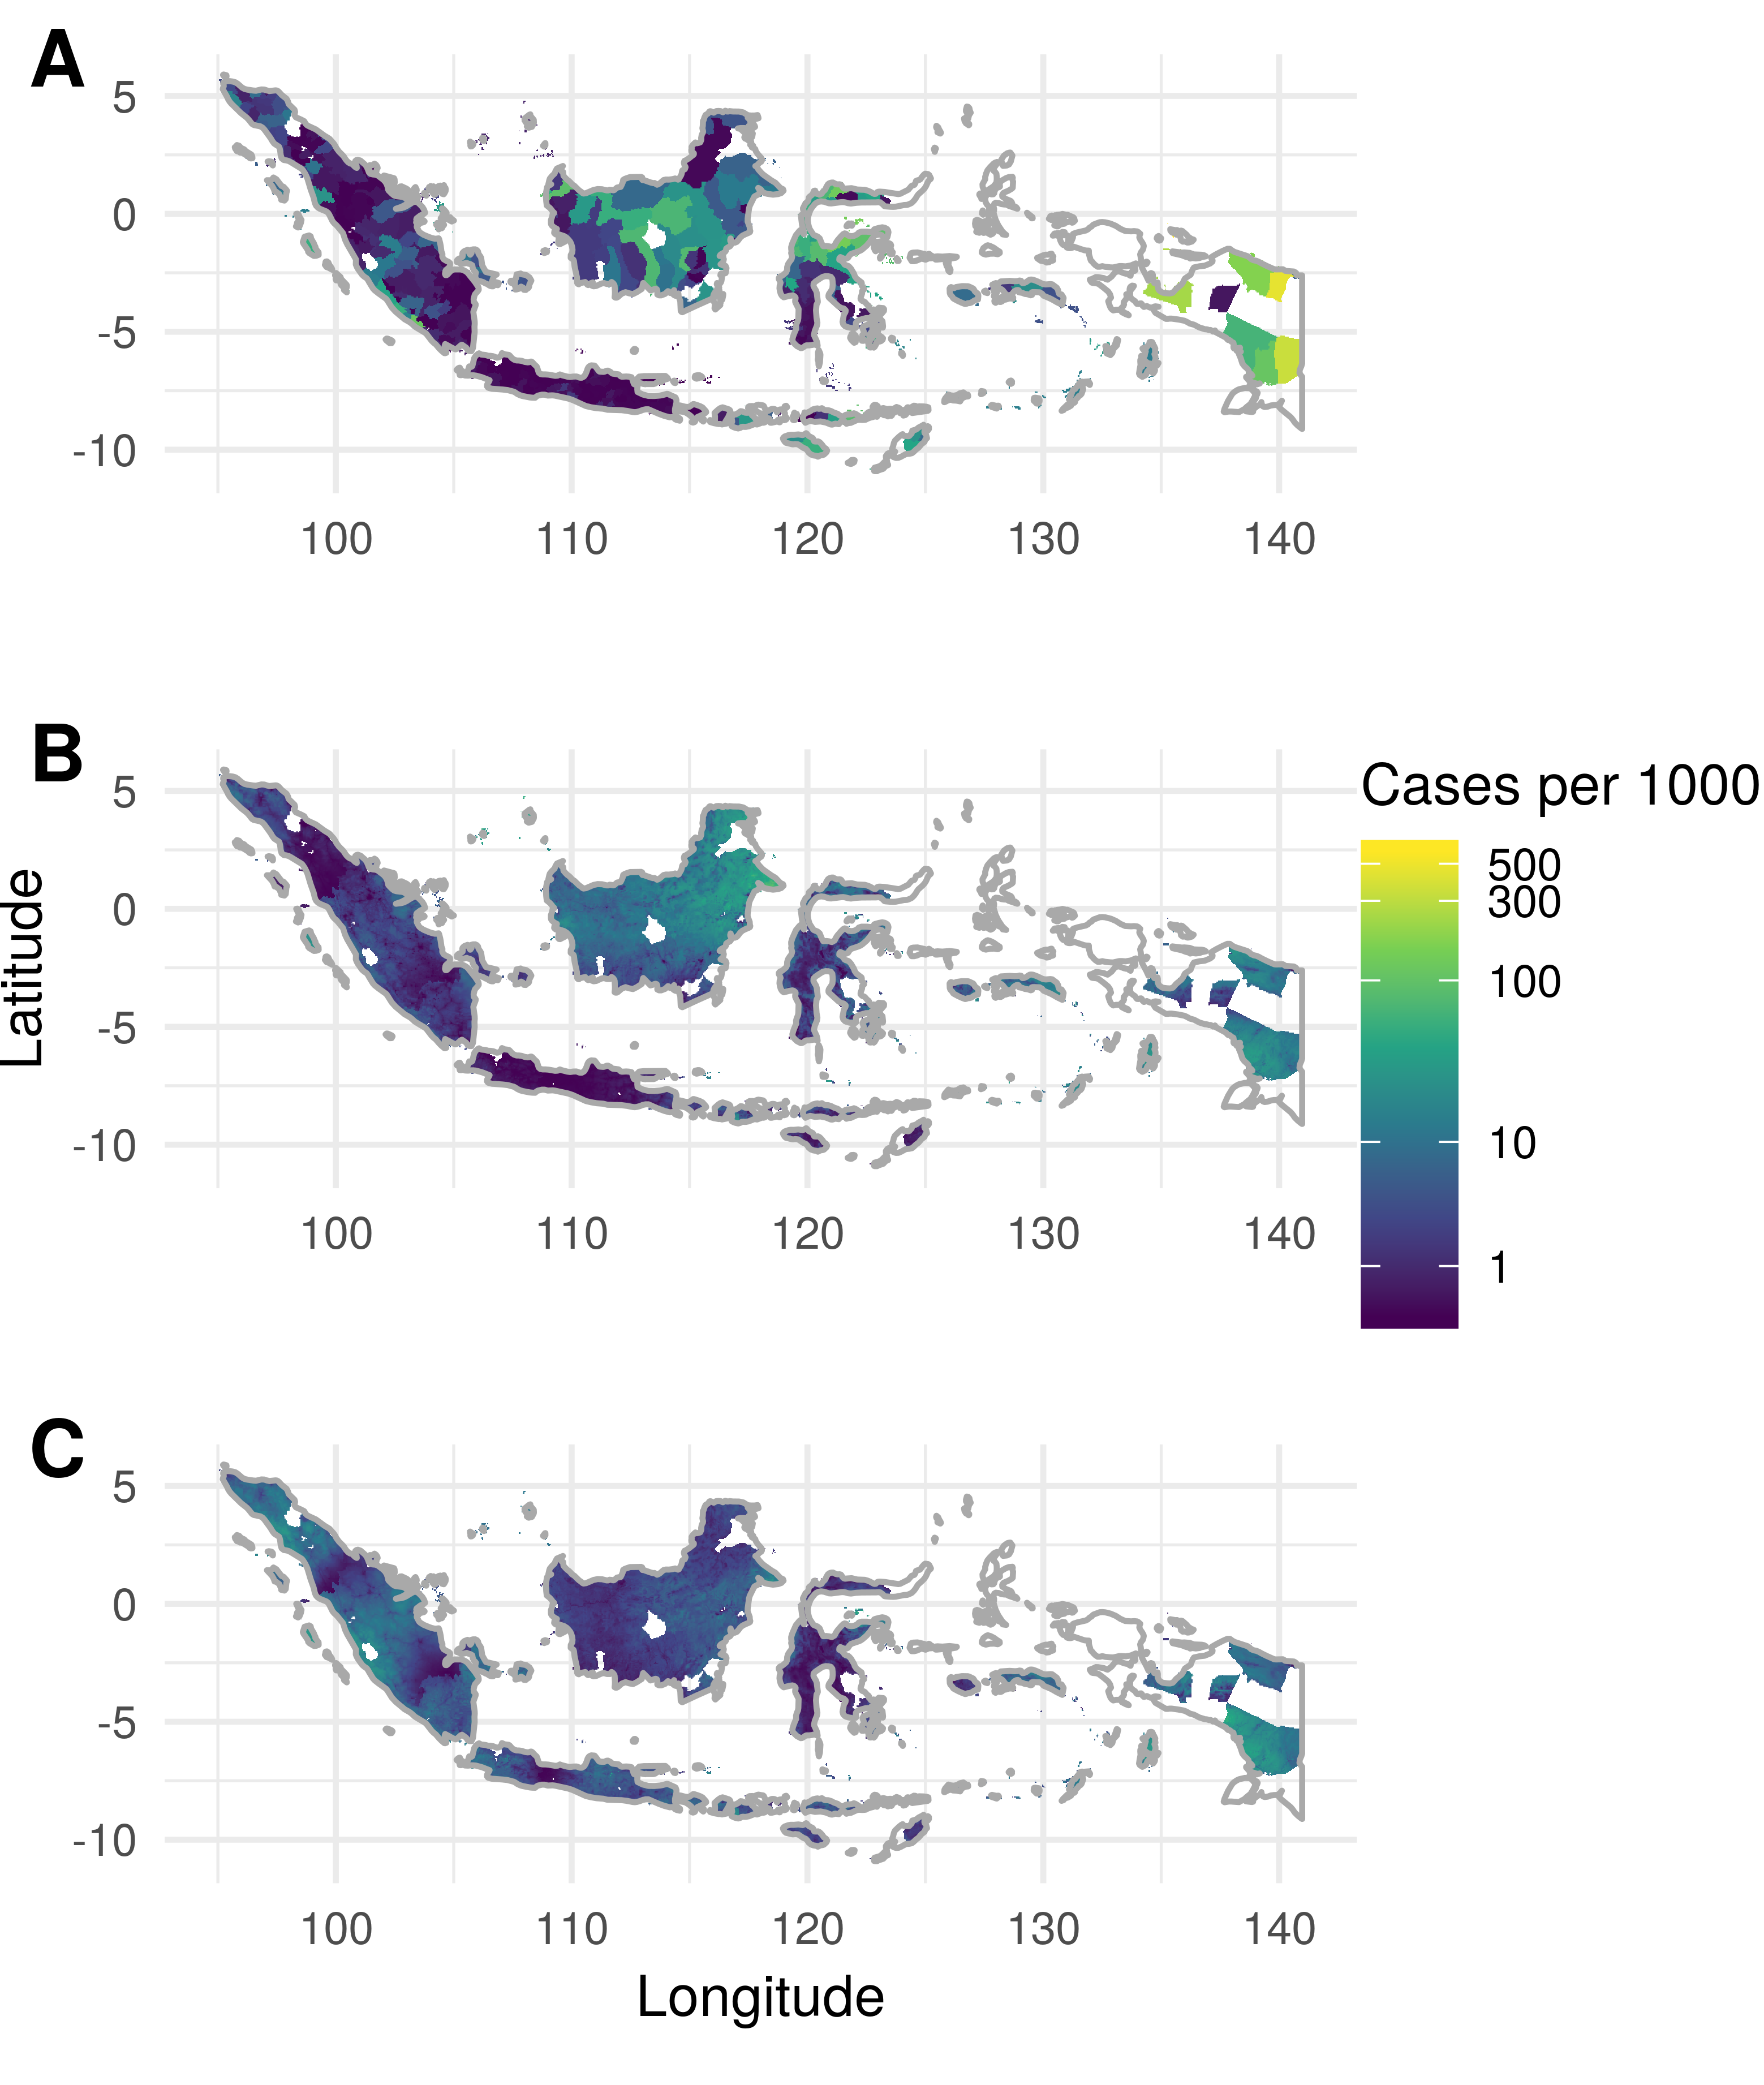
\includegraphics[width = 0.7\textwidth]{figures/idn_both_cv12_preds.png}
%\caption{{\bf Input incidence data and predicted incidence maps. } 
%The incidence (log10) data (top), predicted log10 incidence from the prevalence GP model for spatially sampled out-of-sample polygons (middle) and predicted log10 %incidence from the joint model for spatially sampled out-of-sample polygons (bottom) for Indonesia. The values plotted for areas with no polygon data are the means across all cross-validation folds.
%}
%\label{predobsmapidn}
%\end{figure}






\begin{table}
\caption{\label{table3}Summary of coverage of 80\% credible intervals. The proportion of held out data points that fall within their 80\% credible intervals. 
Cases where this is below 0.7 are highlighted in bold.}
\centering
\fbox{%
\begin{tabular}{lllll}
\hline
{\bf Cross-validation} & {\bf Country}  & {\bf Baseline} & {\bf Prev GP} & {\bf Joint} \\
\hline 
Random & Indonesia  & 0.73 &  0.72 &  0.72\\
& Senegal  & 0.76 &  0.78 &  0.80\\
& Madagascar  & 0.78 &  0.79 &  0.78\vspace{1mm}\\
 Spatial  & Indonesia & 0.71 &  0.72 &  {\bf 0.51}\\
& Senegal  & 0.78 &  0.88 &  0.71\\
& Madagascar  & {\bf 0.67} &  0.70 &  0.72\\
\end{tabular}}
\end{table}


% Results and Discussion can be combined.
%%%%%%%%%%%%%%%%%%%%%%%%%%%%%%%%%%%%%%%%%%%%%%%%%%%%%%%%%%%%%%%%%%%%%%%%%%%%%%%%%%%%%%%%%%%%%%%%%%%%%
\section*{Discussion}
%%%%%%%%%%%%%%%%%%%%%%%%%%%%%%%%%%%%%%%%%%%%%%%%%%%%%%%%%%%%%%%%%%%%%%%%%%%%%%%%%%%%%%%%%%%%%%%%%%%%%


%Summarise results

We have compared the predictive performance (MAE) of three models: a baseline polygon-only model; a disaggregation model with spatial information from prevalence surveys included as an additional covariate from a separate Gaussian process (GP) model; and a model that jointly learns from polygon incidence data and prevalence point-surveys.
The prevalence GP model never performed worse than baseline and performed better than baseline in one case.
The joint model performed best in one case but also performed worse than baseline in two cases.
Therefore, fitting a spatial Gaussian process to prevalence points and including these predictions seems to be a more reliable way of using spatial information from prevalence points.
However, given that this comparison was conducted on datasets from only three countries, it is challenging to draw firm conclusions.
The significant differences between models all occurred under spatial cross-validation.
This implies that the models are not using the additional data to learn more accurate relationships between the environment and malaria incidence. 
Instead it suggests that the models are using the spatial information in the data to improve predictions.

% joint model benefits
% robust
% lower sd of posteriors
% learn relationship
% disappointed that we couldn't get it to out perform

A full joint model using both prevalence surveys and incidence data gains additional statistical power compared to the baseline or prevalence GP models.
Therefore, it is worth considering why the performance of this model was generally less good than the simpler prevalence GP model that did not benefit from the additional statistical power.
One potential reason is that the malariometric data are on different scales.
Here we have used a previously fitted model \citep{cameron2015defining} to inform the joint model.
However, this model was calibrated using relatively few matched prevalence and incidence surveys as few of these have been conducted and published.
Although we added the parameter $\alpha$ that scales this relationship, it is a very simple scaling.
Furthermore the true relationship between prevalence and incidence is likely to vary spatially as aspects such as immunity, seasonality, and population age-structure are not constant \citep{cameron2015defining, battle2015defining, reiner2015seasonality}.
In using a joint model we are accepting these limitations in the hope that the benefits of including additional data outweigh the costs of using mismatched data.

In our sensitivity analysis we found that changing the coefficients in the relationship considerably reduced predictive ability (though weakening the prior on $\alpha$ did not). 
We might interpret this as suggesting that the prior was too strong but that as the data did not contradict the prior relationship, this did not matter.
Future models could potentially be improved by using a more flexible approach for addressing the shortcomings of the prevalence-incidence relationship \citep{cameron2015defining} being used in this context.
This could be by estimating the parameters of the polynomial jointly with the rest of the model.
Informative priors based on the original model could be used to regularise this joint fit both to prevent improbable inferences but also because if the relationship were too flexible, the information from the prevalence data might not contribute to informing the regression parameters and spatial random field.
This is particularly true for model forms such as a spline or a Gaussian process on the relationship between prevalence and incidence.
For the model to handle noisy or biased prevalence point-surveys, the modeller can control the iid random effect on the point-surveys, $w_b$ and the prevalence intercept $\beta_p$. 
Here we have tried to maximise the influence of the prevalence data by setting the prior based on the belief that the random effect should only explain extra-binomial variation that is impossible to derive from the covariates (e.g. based on the differences in prevalence surveys within the same pixel).
Weakening this prior will allow the iid effect to explain more of the prevalence point-survey variation which both reduces the potential statistical power gained by adding the point-surveys but also reduces the effects of biased or noisy estimates.

In this research we have used only linear covariates but previous work has demonstrated that simple linear combinations of environmental covariates cannot fully explain malaria risk \citep{bhatt2017improved}.
A number of methods could be used to include non-linear effects of covariates and interactions into the model.
Firstly, machine learning models could be fitted to the prevalence data and then predictions from these models could be used as covariates in the full model \citep{bhatt2017improved}.
This approach is feasible but would not allow any information from the polygons to inform non-linear relationships.
Directly modelling non-linear effects in the full model could be achieved by including simple non-linear functions such as splines \citep{sissoko2017temporal, sewe2017using, hundessa2018projecting}, though the increased model complexity would require more data than was used in Senegal and Madagascar in this study.
Finally, Gaussian process regression, with smoothly varying effects in environmental and geographic space could be used \citep{law2018variational}.
Unfortunately, each of these options is computationally expensive without variational Bayes or other approximations \citep{law2018variational, ton2018spatial}, which can be difficult to derive.
Additionally these models require a large volume of response data and careful regularisation for good predictive performance.

We used three case studies, limited by the number of countries with good aggregated incidence data as well as good prevalence survey data.
Two types of study region seemed likely to benefit from the methods presented here.
First, countries like Madagascar with intermediate transmission intensities and good surveillance data and good prevalence data.
Second, countries that have lots of prevalence surveys and are adjacent to countries with good reporting systems, (e.g. Papua New Guinea and neighbouring Indonesia), might also benefit from models that share information between countries.
Given the small number of case studies it is hard to determine in which countries these methods are likely to be most effective.
However, the benefits here were only seen in spatial cross-validation schemes suggesting that the models were only effectively using spatial information.



%%%%%%%%%%%%%%%%%%%%%%%%%%%%%%%%%%%%%%%%%%%%%%%%%%%%%%%%%%%%%%%%%%%%%%%%%%%%%%%%%%%%%%%%%%%%%%%%%%%%%
\section*{Conclusion}
%%%%%%%%%%%%%%%%%%%%%%%%%%%%%%%%%%%%%%%%%%%%%%%%%%%%%%%%%%%%%%%%%%%%%%%%%%%%%%%%%%%%%%%%%%%%%%%%%%%%%


We have presented two methods for combining spatial information from prevalence surveys with disaggregation regression models.
We found that while the predicted maps were quite different, the polygon-level predictive performance was usually not significantly different.
The prevalence GP model never performs worse than baseline and performs better than baseline in one case. 
The full joint model performs worse than baseline in two cases but is the best performing model in one case.
As more countries produce reliable routine surveillance data, and as more countries reduce their malaria prevalences to the point where prevalence surveys are no longer sensitive, disaggregation regression will become more commonly used. 
Methods such as those presented here should be explored further and refined to improve disaggregation regression results where and when the requisite data are available.



\section*{Supporting information}


\section*{Acknowledgments}
The authors acknowledge the National Malaria Control Programme of Madagascar for sharing their routine case data for this analysis.


%\bibliographystyle{apalike} %or any other style you like

\bibliographystyle{rss}


\bibliography{Malaria} 



\end{document}

